% THIS IS SIGPROC-SP.TEX - VERSION 3.1
% WORKS WITH V3.2SP OF ACM_PROC_ARTICLE-SP.CLS
% APRIL 2009
%
% It is an example file showing how to use the 'acm_proc_article-sp.cls' V3.2SP
% LaTeX2e document class file for Conference Proceedings submissions.
% ----------------------------------------------------------------------------------------------------------------
% This .tex file (and associated .cls V3.2SP) *DOES NOT* produce:
%       1) The Permission Statement
%       2) The Conference (location) Info information
%       3) The Copyright Line with ACM data
%       4) Page numbering
% ---------------------------------------------------------------------------------------------------------------
% It is an example which *does* use the .bib file (from which the .bbl file
% is produced).
% REMEMBER HOWEVER: After having produced the .bbl file,
% and prior to final submission,
% you need to 'insert'  your .bbl file into your source .tex file so as to provide
% ONE 'self-contained' source file.
%
% Questions regarding SIGS should be sent to
% Adrienne Griscti ---> griscti@acm.org
%
% Questions/suggestions regarding the guidelines, .tex and .cls files, etc. to
% Gerald Murray ---> murray@hq.acm.org
%
% For tracking purposes - this is V3.1SP - APRIL 2009
\documentclass{acm_proc_article-sp}
\usepackage[slovene]{babel}
\usepackage[utf8]{inputenc}
\usepackage{url}

\begin{document}

\title{Analiza podatkov VoIP klicev}
\subtitle{[Članek pri predmetu Digitalna forenzika]
%\titlenote{A full version of this paper is available as
%\textit{Author's Guide to Preparing ACM SIG Proceedings Using
%\LaTeX$2_\epsilon$\ and BibTeX} at
%\texttt{www.acm.org/eaddress.htm}}}
}

%
% You need the command \numberofauthors to handle the 'placement
% and alignment' of the authors beneath the title.
%
% For aesthetic reasons, we recommend 'three authors at a time'
% i.e. three 'name/affiliation blocks' be placed beneath the title.
%
% NOTE: You are NOT restricted in how many 'rows' of
% "name/affiliations" may appear. We just ask that you restrict
% the number of 'columns' to three.
%
% Because of the available 'opening page real-estate'
% we ask you to refrain from putting more than six authors
% (two rows with three columns) beneath the article title.
% More than six makes the first-page appear very cluttered indeed.
%
% Use the \alignauthor commands to handle the names
% and affiliations for an 'aesthetic maximum' of six authors.
% Add names, affiliations, addresses for
% the seventh etc. author(s) as the argument for the
% \additionalauthors command.
% These 'additional authors' will be output/set for you
% without further effort on your part as the last section in
% the body of your article BEFORE References or any Appendices.

\numberofauthors{2} %  in this sample file, there are a *total*
% of EIGHT authors. SIX appear on the 'first-page' (for formatting
% reasons) and the remaining two appear in the \additionalauthors section.
%
\author{
% You can go ahead and credit any number of authors here,
% e.g. one 'row of three' or two rows (consisting of one row of three
% and a second row of one, two or three).
%
% The command \alignauthor (no curly braces needed) should
% precede each author name, affiliation/snail-mail address and
% e-mail address. Additionally, tag each line of
% affiliation/address with \affaddr, and tag the
% e-mail address with \email.
%
% 1st. author
\alignauthor Tomaž Tomažič\\
       \affaddr{Fakulteta za računalništvo in infromatiko}\\
       \affaddr{Tržaška 25}\\
       \affaddr{Ljubljana, Slovenia}\\
       \email{tt3710@student.uni-lj.si}
% 2nd. author
\alignauthor Zupanec Žiga\\
       \affaddr{Fakulteta za računalništvo in infromatiko}\\
       \affaddr{Tržaška 25}\\
       \affaddr{Ljubljana, Slovenia}\\
       \email{zz9698@student.uni-lj.si}
% % 3rd. author
% \alignauthor Lars Th{\o}rv{\"a}ld\titlenote{This author is the
% one who did all the really hard work.}\\
%        \affaddr{The Th{\o}rv{\"a}ld Group}\\
%        \affaddr{1 Th{\o}rv{\"a}ld Circle}\\
%        \affaddr{Hekla, Iceland}\\
%        \email{larst@affiliation.org}
% \and  % use '\and' if you need 'another row' of author names
% % 4th. author
% \alignauthor Lawrence P. Leipuner\\
%        \affaddr{Brookhaven Laboratories}\\
%        \affaddr{Brookhaven National Lab}\\
%        \affaddr{P.O. Box 5000}\\
%        \email{lleipuner@researchlabs.org}
% % 5th. author
% \alignauthor Sean Fogarty\\
%        \affaddr{NASA Ames Research Center}\\
%        \affaddr{Moffett Field}\\
%        \affaddr{California 94035}\\
%        \email{fogartys@amesres.org}
% % 6th. author
% \alignauthor Charles Palmer\\
%        \affaddr{Palmer Research Laboratories}\\
%        \affaddr{8600 Datapoint Drive}\\
%        \affaddr{San Antonio, Texas 78229}\\
%        \email{cpalmer@prl.com}
}
% There's nothing stopping you putting the seventh, eighth, etc.
% author on the opening page (as the 'third row') but we ask,
% for aesthetic reasons that you place these 'additional authors'
% in the \additional authors block, viz.
% additionalauthors{Additional authors: John Smith (The Th{\o}rv{\"a}ld Group,
% email: {\texttt{jsmith@affiliation.org}}) and Julius P.~Kumquat
% (The Kumquat Consortium, email: {\texttt{jpkumquat@consortium.net}}).}
\date{30 July 1999}
% Just remember to make sure that the TOTAL number of authors
% is the number that will appear on the first page PLUS the
% number that will appear in the \additionalauthors section.

\maketitle
\begin{abstract}
Popularnost telefonije preko IP (VoIP) je v zadnjih letih narasla, ker je cenovno ugodnejša in enostavnejša za uporabo. Kakorkoli že, ta tehnologija je tudi atraktivna za kriminal, ker je VoIP globalna telefonska storitev, v kateri je težko identificirati uporabnika. Privlačna je tudi zaradi visoke varnosti, saj veliko implementacij uporablja močno enkripcijo za zaščito, tako zvočnih podatkov kot kontrolo samih sporočil v primerjavi z žično telefonijo kjer je prisluškovanje enostavnejše. Zato so za VoIP klice potrebni drugi načini pridobivanja digitalnih dokazov in informacij. V najini raziskavi smo pogledali kateri dokazi ostanejo po opravljenem VoIP klicu na obeh napravah, trdem disku in bralno-pisalnem pomnilniku (RAM).

\end{abstract}

% % A category with the (minimum) three required fields
% \category{H.4}{Information Systems Applications}{Miscellaneous}
% %A category including the fourth, optional field follows...
% \category{D.2.8}{Software Engineering}{Metrics}[complexity measures, performance measures]

\keywords{Digitalna forenzika, dokazi, telefonija preko IP, VoIP, forenzika v pomnilniku} % NOT required for Proceedings

\section{Uvod}
VoIP telefonija je tehnologija preko katere se prenaša večpredstavnostna vsebina po internetnem omrežju. Uporablja močno enkripcijo za zaščito, tako zvočnih podatkov kot kontrolo samih sporočil v primerjavi z žično telefonijo kjer je prisluškovanje enostavnejše. Zato so za VoIP klice potrebni drugi načini pridobivanja digitalnih dokazov in informacij. V najini raziskavi smo pogledali kateri dokazi ostanejo po opravljenem VoIP klicu na obeh napravah, trdem disku in bralno-pisalnem pomnilniku (RAM).

Identifikacijske poverilnice so osnovane v informacijah iz glav paketov vsebovanih v VoIP protokolu. Narejeni so bili različni kontrolni testi v katerih je bila forenzična analiza narejena na virtualnih strojih s katerimi so bili opravljeni različni VoIP klici. Eksperimenti so bili ponovljeni na istem protokolu tako na disku kot v bralno pisalnem pomnilniku (RAM).

\section{Paleta VoIP}
Telefonija preko IP protokola je zelo spremenila način kako se podatki telefoniranja prenašajo in tako začela pravo telekomunikacijsko industrijo. S samo rastjo popularnosti in široko dostopnostjo do interneta je omogočeno, da se klici prenašajo preko internetne infrastrukture kot pa po tradicionalnem javno komutiranem telefonskem omrežju (PSTN). Ta tehnologija, ki se ji reče VoIP, uporablja internetni protokol (IP) za prenašanje paketov ki vsebujejo majhne koš-čke glasovnega pogovora med klicočima.

Popularnost VoIP je narasla zaradi cenejše in enostavnejše uporabo tako doma kot v podjetjih\cite{ORIG}. Kakorkoli že, ta tehnologija je zelo privlačna za kriminalce, še posebej za VoIP pogovore ki niso spremljani iz strani internetnega ponudnika. To je zaradi tega ker je VoiP globalen telefonski servis v katerem je težko identificirati uporabnikovo identiteto, ker večina implementacij uporablja močno enkripcijo za zavaro\-vanje tako zvočnih podatkov kot kontrolo samih sporočil in nadziranje ali sledenje takšnih VoIP klicev je oteženo zaradi konvencionalnih metod kot so žično prisluškovanje in le teh ni mogoče aplicirati na VoIP klice. Zaradi teh razlogov so za pridobivanje podatkov in informacij iz telefonije preko IP potrebne druge metode. Bistveno za forenzične raziskovalce je, da imajo metodo ki omogoča organom pregona premagati nekatere vidike tega načina telefonije, ki so ugodne za storilce kaznivih dejanj.

Ta uvod podaja pregled transportnih protokolov VoIP in signalne protokole. Ti določajo podatke, iz katerih je mogoče forenzično pridobiti polja iz glave protokola, kot tudi uporabnikovo registracijo za VoIP klic.

VoIP ni samo en protokol ampak kolekcija različnih že obstoječih protokolov, ki so uporabljeni za vzpostavitev, vzdrževanje in končanje klica, protokoli za enkapsulacijo in prenos paketov po internetu.
Protokoli IP, UDP in RTP so protokoli ki enkapsulirajo in prenašajo pakete, ki vsebujejo informacije potrebne za identifikacijo izvora in ponora klicateljev in dostavo samih zvočnih podatkov. Session Initiation Protocol (SIP) je signalni protokol uporabjen za vzpostavitev, vzdrževanje in zaključevanje klica.


\subsection{Internet Protocol}

Protokol IP\cite{IP} je odgovoren za hranjenje internetnega naslova v glavi, kar omogoča paketom da so dostavljeni iz svojega izvora do IP naslova. Format glave protokola IP je prikazan na sliki~\ref{fig:ip}.

\begin{figure}
\centering
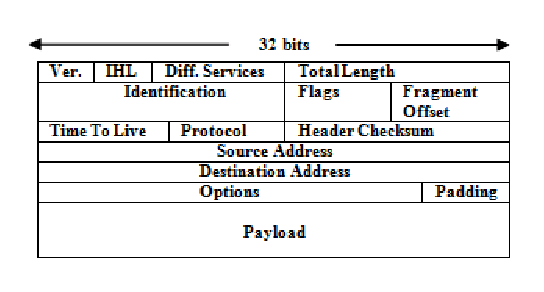
\psfig{file=semi_slike/IP_packet.eps,} % height=1in, width=1in,}
\caption{Format glave paketa IP.}
\label{fig:ip}
\end{figure}


\subsection{User Datagram Protocol}
Zanesljiv protokol za prenos paketov po internetu je protokol TCP\cite{TCP}, ki zagotavlja dostavo tudi za izgubljene in pokvarjene pakete s ponovnim pošiljanjem. Vendar za VoIP klice, ki potekajo v realnem času, ni smisla ponovnega pošiljanja za izgubljene pakete. TCP uporablja nadzor pretoka, ki začasno zaustavi prenos paketov dokler pokvarjeni paket ni uspešno prenešen.

Namesto protokola TCP je za zahteve VoIP bolj primeren, čeprav je manj zanesljiv pri dostavi paketov, protokol UDP (slika~\ref{fig:udp}). Izbran sistem je tako sklad protokola IP/UDP. IP datagram zagotavlja izvorni in ciljni naslov in izvorna in ciljna vrata. Pogoste aplikacije delujejo na specifičnih vratih. Ker TCP zagotavlja prenos izgubljenih paketov, ni zaželjen v realnočasnih aplikacijah in je zato za prenos zvoka uporabljen UDP.

\begin{figure}
\centering
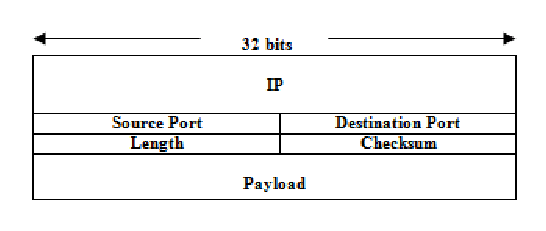
\psfig{file=semi_slike/UDP_packet.eps,} % height=1in, width=1in,}
\caption{Glava paketa UDP.}
\label{fig:udp}
\end{figure}

Protokol UDP\cite{UDP} se uporablja tudi zaradi lažjega prebijanja NAT-a pri uporabi načina prevajanje omrežnega naslova (angl. Network Address Translation, krat. NAT). Poznamo več vrst NAT (slika~\ref{fig:nat}) in sicer:
\begin{itemize}
  \item Direktna preslikava (angl. Full-cone) pri kateri se notranji lokalni IP naslov in vrata preslikajo v zunanji IP naslov z istimi vrati. Zunanji odjemalci lahko s pošiljanjem na začasni par (zunaj vidni IP naslov in vrata) pošiljajo sporočila notranjemu IP naslovu.
  \item Omejena direktna presilava (angl. Restricted cone): deluje na istem principu kot direktna preslikava z omejitvijo, da mora prvi paket poslati interni odjemalec.
  \item Z vrati omejena direktna preslikava: zunanji odjemalec lahko pošlje paket le na vrata, katerim je predhodno pošiljal notranji odjemalec.
  \item Simetrična preslikava (angl. Symmetric cone): usmerjevalnik vodi preslikovalno tabelo glede na ponorni IP naslov in vrata. Vrata se dodelijo naključno za čas trajanja seje glede na ponorni IP naslov. Le tisti zunaji odjemalec, ki prejme paket paket notranjega odjemalca lahko pošlje paket nazaj (odgovori) notranjemu odjemalcu.
\end{itemize}

\begin{figure}
\centering
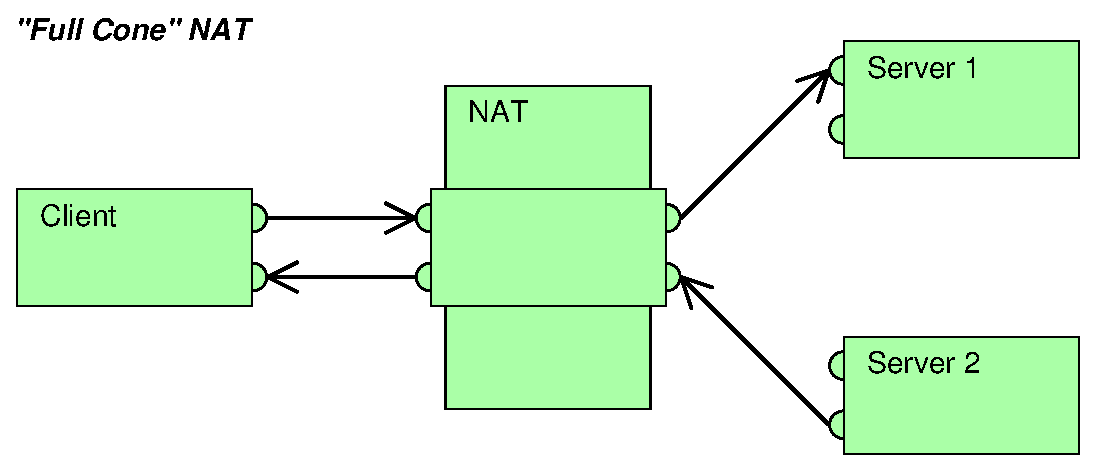
\psfig{file=semi_slike/Full_Cone_NAT.eps, width=3in,} % height=1in, width=1in,}
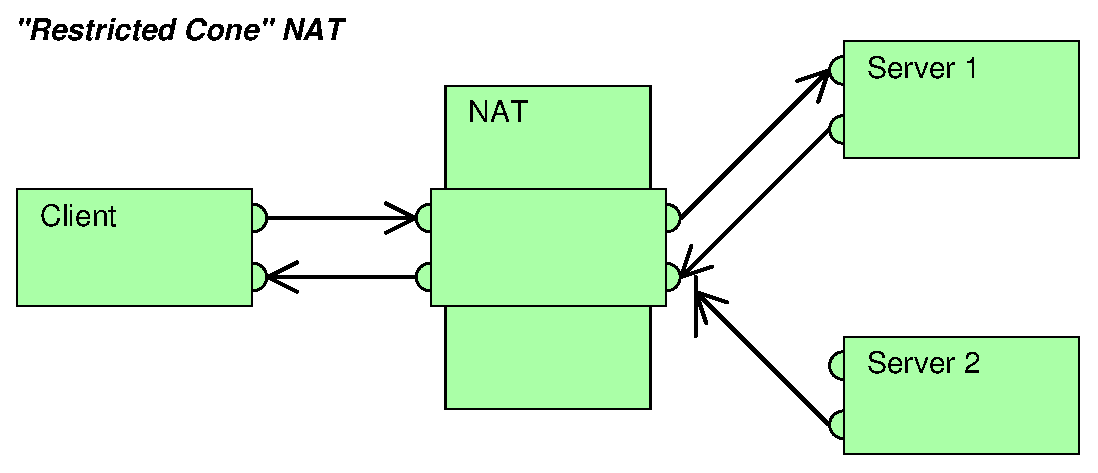
\psfig{file=semi_slike/Restricted_Cone_NAT.eps, width=3in,} % height=1in, width=1in,}
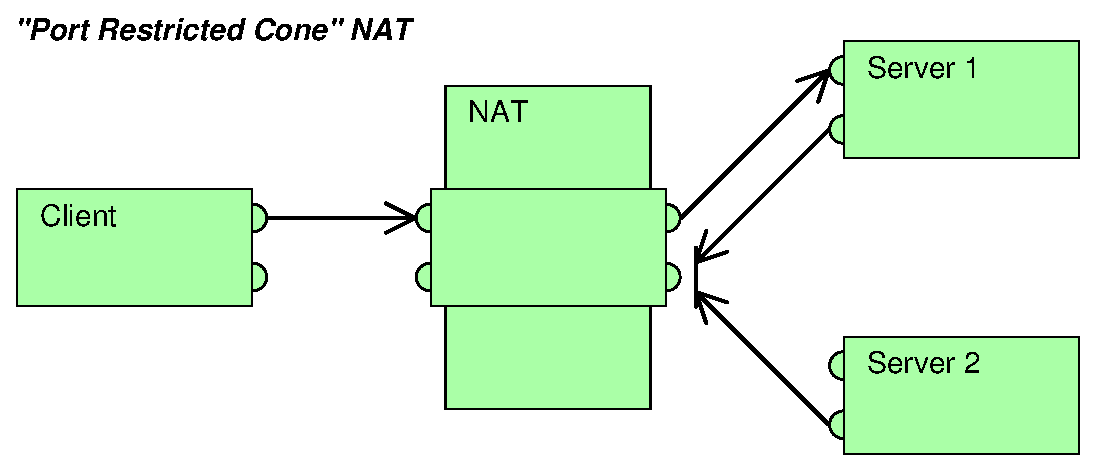
\psfig{file=semi_slike/Port_Restricted_Cone_NAT.eps, width=3in,} % height=1in, width=1in,}
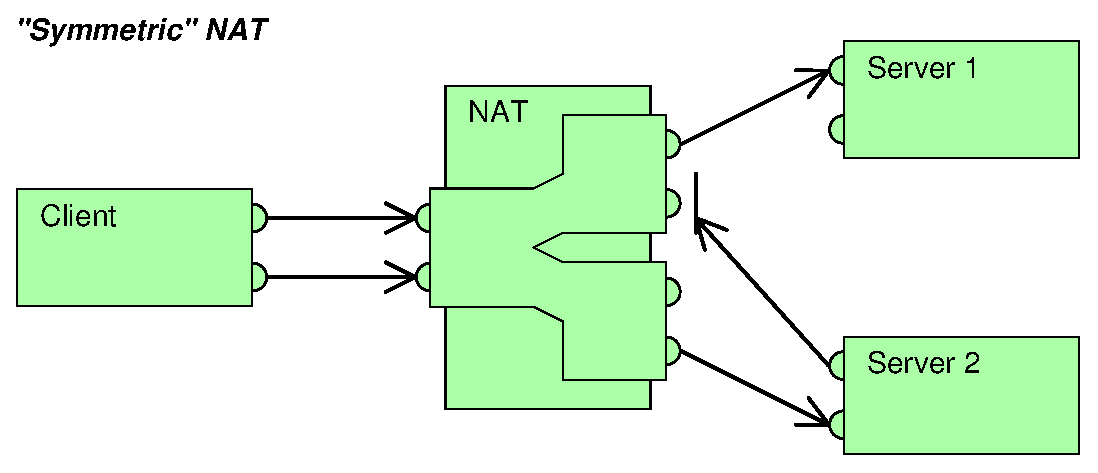
\psfig{file=semi_slike/Symmetric_NAT.eps, width=3in,} % height=1in, width=1in,}
\caption{Primerjava med različnimi metodami NAT.}
\label{fig:nat}
\end{figure}

NAT prebijamo\cite{NAT-FIREWALL} z orodji za sprehajanje po takih omrežjih, ki jih imenujemo ''Obhod NAT-a'', (angl. Session Traversal Utilities for NAT, krat. STUN\cite{STUN}). Gre za tehniko, ki vzpostavi in vzdržuje IP povezave skozi NAT usmerjevalnike, ki kršijo povezavo iz enega konca na drugi (end-to-end). Uporablja se za peer-to-peer in VoIP povezave. Obstaja veliko metod za rešitev tega problema, vendar ne obstaja ena univerzalna. Metoda, pri kateri potrebujemo strežnik, se imenuje "relay" oz. posrednik. Pri takem načinu, potujejo paketi enega odjemalca najprej do strežnika, ki jih nato posreduje drugemu odjemalcu in obratno. Streznik mora biti naprava s katero lahko komunicirata oba odjemalca, ki sta v omrezju NAT. Veliko tehnik uporablja pomoč strežnika. Nekatere pa strežnik uporabljajo samo za vzpostavitev povezave. Če strežnik uporabljajo za celotno komunikacijo se s tem zniža kvaliteta povezave in poveča latenca. Druga tehnika je, da se dovoli požarnim zidovom in NAT omrežjem da dopuščajo VoIP, hkrati pa ohranjajo varnost podjetij. To določajo protokoli RSIP (realm-specific IP) in MIDCOM (middlebox communications).

\subsection{Real-Time Transport Protocol}

Real-Time Transport Protocol (RTP) zagotavlja prometno omrežje za aplikacije v realnem času, kot so prenos zvoka preko paketno komutiranega omrežja. Protokol RTP je izbran za prenos govornih podatkov, saj dodaja dodatne informacije, kot je na primer zaporedna številka za vsak paket, da zagotovijo prejemni aplikaciji zvoka možnost razporeditve paketov v pravilnem vrstnem redu in zagotavlja tudi časovno oznako za vsak posamezen paket, ki omogoča predvajanje zvoka v zaporednih časovnih presledkih. Za klicanje in sprejemanje VoIP klica ni potrebna uporaba protokola RTP, vendar ta lahko preprosto doda dodatne podatke, ki pripomorejo k sprejemanju paketov v vrstnem redu in olajša delo z VoIP konferencami. Sklad IP/UDP/RTP in glava paketa RTP je prikazana na sliki~\ref{fig:ip-udp-rtp}.

\begin{figure}
\centering
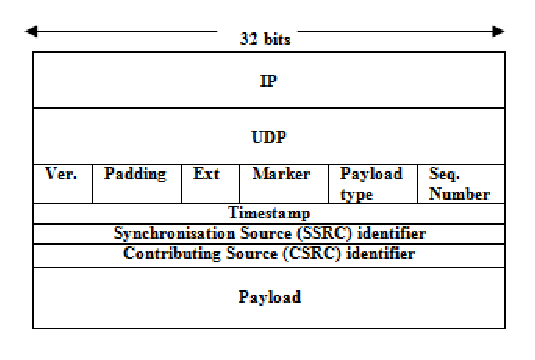
\psfig{file=semi_slike/ip_udp_rtp.eps,} % height=1in, width=1in,}
\caption{Sklad UDP/RTP in glava paketa RTP.}
\label{fig:ip-udp-rtp}
\end{figure}

Za vsak paket sta enolično določena časovna značka in sekv\-enčna številka. Sekvenčna številka se poveča z vsakim poslanim paketom in omogoča ponovno razvrstitev in detekcijo izgube paketov na prejemnikovi strani.

Polje sinhronizacijski izvorni identifikator (SSRC) označuje izvor sinhronizacije, navadno z računalnikovo uro medtem ko polje doprinašani izvor (CSRC) označuje vir posameznih prispevkov, ki sestavljajo en podatkovni tok paketov. Za sodelovanje v VoIP klicu ni nujno uporabljati protokola RTP. Nekatere aplikacije VoIP kot je na primer Skype ne uporabljajo protokola RTP, medtem ko pa ga X-Lite in Ekiga\cite{EKIGA} uporabljajo. Prav zaradi tega smo naš eksperiment naredili na programu Ekiga saj imamo z dodatnim protokolom RTP, potem na voljo dodatna polja iz katerih lahko iščemo informacije o klicu.

Zvočni posnetek je razdeljen v paket ki je potem prenesen po omrežju. Če je paket prevelik in ga je potrebno fregmenitrati ali pa izvira iz različnih virov, potem bo imel vsak fragment enak CSRC za identifikacijo izvora iz istega podatkovnega toka. Različne sekvenčne števlike pa omogočajo rekonstrukcijo v pravem zaporedju za vsak CSRC. To je uporabljeno za sinhronizacijo na prejemnikovi strani.


\subsection{SIP protocol}

Protokol SIP\cite{SIP} omogoča klicanje uporabniških posrednikov (UA) za lokacijo in registracijo z uporabo proxy strežnikov, ki omogočajo drugim uporabniškim posrednikom priključitev v klicno sejo. Vsaka transakcija je sestavljena iz zahteve, ki sproži določeno metodo na vsaj en odgovor, kot je prikazano na sliki~\ref{fig:sip}. Jane uporablja svojo VoIP aplikacijo za pošiljanje zahteve Invite (vabilo) Joetu. Zahteva Invite je SIP metoda, ki določa akcije, ki jih Jane želi od Joeta, to je sprejetje klica. Zahteva Invite gre skozi dva proxy strežnika, da doseže Joeta (korak od 1 – 5). Na prejemnikovi strani se začne zvonjenje, odgovor pa Joe vrne pošiljatelju ponovno skozi oba proxy strežnika (korak 6 – 8). Joe potrdi prejetje zahtevka Invite z odgovorom OK osebi Jane (9 – 11). Prenos večpredstavnostne vsebine se začne ko Jane potrdi odgovora OK (12). Ta sejo lahko zaključi katerikoli udeleženec v komunikaciji (13 -14).

\begin{figure}
\centering
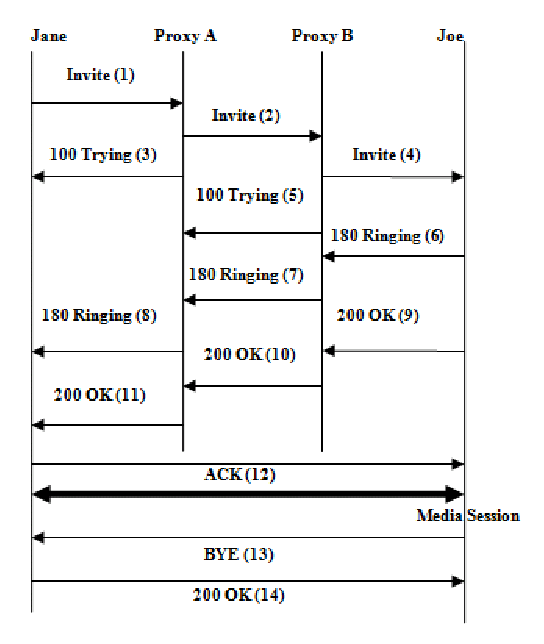
\psfig{file=semi_slike/SIP_session.eps,} % height=1in, width=1in,}
\caption{Primer izmenjave sporočil med sejo SIP.}
\label{fig:sip}
\end{figure}

\section{Alternativni protokoli VoIP}
Vrata, ki se navadno uporabljajo pri paleti protokolov VoIP so povzeta v tabeli~\ref{fig:ports}.

\begin{table*}
\centering
\caption{Uporaba vrat pri protokolu VoIP}
\label{fig:ports}
\begin{tabular}{|c|c|l|l|} \hline
  Protokol&Vrata&Tip&Razlaga\\ \hline
  SIP & 5000 do 5100& UDP & SIP seja privzeto 5060. Različno pri NAT.\\ \hline
  STUN & 3478 do 3479& UDP & \\ \hline
  RTP & Naključna/razpoložljiva & UDP & Prihajajoč promet na drugi strani. Navadno 5004, 7070, 16382\\ \hline
  H.323 & 1720 & TCP & Poslušanje.\\ \hline
  H.323 & 5000 do 5100 & UDP & Vratarji.\\ \hline
  H.323 & 30000 do 30010 & TCP & Kanal H.245 za Microsoft Netmeeting.\\
\hline\end{tabular}
\end{table*}

\subsection{Paleta protokolov H.323}

Namesto protokola SIP se lahko za vzpostavitev seje, kontrolo nad sejo, prenos multimedijskih podatkov in kontrolo pasovne širine uporabi zbirka tehnologij H.323 (slika~\ref{fig:h323}). H.323 \cite{H323} lahko po funkcionalnosti grobo primerjamo s protokolom SSL/TLS, a je precej obsežnejši. Protokol povezuje različne naprave (terminale, usmerjevalnike (angl. MCUs), prehode vratarje, in zaključne elemente).

Terminali so naprave katere tipično uporablja končni uporabnik (telefoni, programski odjemalci, konferenčni sistemi ...). Usmerjevalniki povezujejo oziroma združujejo terminale ali skupino le-teh med seboj. Prehodi skrbijo za združljivost med različnimi tehnologijami, ki se uporabljajo pri povezovanju naprav (PTSN, ISDN). Vratarji niso obvezni za delovanje sistema skrbijo pa za registracijo končnih naprav, avtentikacijo uporabnikov, preslikavo naslovov, dovoljenja uporabnikov in/ali naprav. Vratarji med seboj uporabljajo protokol RAS (angl. Remote Access Service). Zaključni elementi prav tako niso potrebni, uporabljajo pa se za nadzor, upravljanje terminalov in vodenje računov znotraj upravljalske domene. Po analogiji spominjajo na naprave RAS\footnote{Ni enako kot prej omenjeni RAS (Registration, Admission and Status).} (angl. Remote Access Server) \cite{RAS}.

\begin{figure}
\centering
\psfig{file=semi_slike/h323_stack.eps, width=3in,} % height=1in, width=1in,}
\caption{Celoten sklad protokola H.323.}
\label{fig:h323}
\end{figure}

%-----------------
% Ni enako kot prej omenjeni RAS (Registration, Admission and Status).


\subsubsection{Primer vzpostavitve klica}

\begin{figure}
\centering
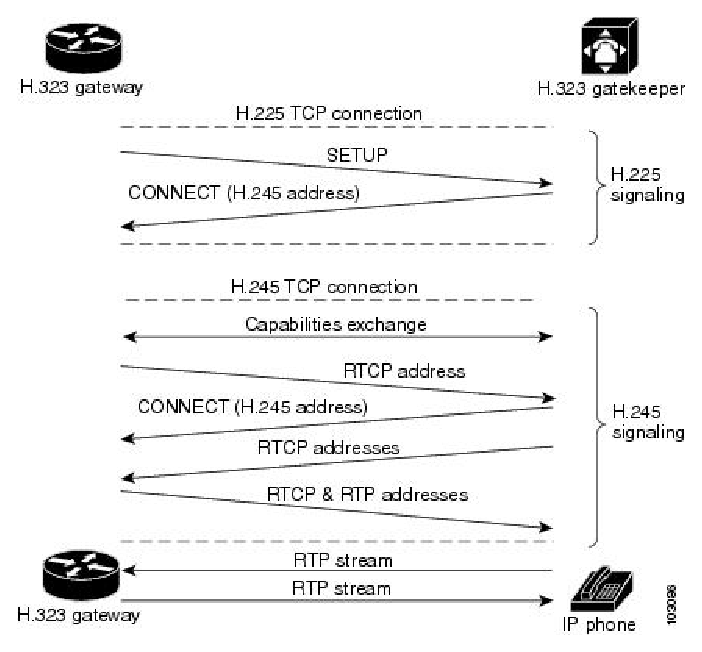
\psfig{file=semi_slike/h323_signaling.eps, width=3in,} % height=1in, width=1in,}
\caption{Primer vzpostavitve klica pri protokolu H.323.}
\label{fig:h323-call}
\end{figure}

Faze pri vzpostavitvi klica pri protokolu H.323 (slika~\ref{fig:h323-call}).
\begin{enumerate}
  \item Setup (Namera o vzpostavitvi povezave z napravo.)
  \item Setup acknowledge (Klicana naprava želi komunicirati s klicočo.)
  \item Call Porceeding (Potrditev klicane naprave, da ima vse potrebne informacije za usmeritev klica.)
  \item Progress (Obvestilo prehoda, da klic v izvajanju.)
  \item Alerting (Obvestilo klicane naprave, da je pričela z zvonenjem.)
  \item Connect (Obvestilo klicane naprave, da je klic sprejet - uporabnik je dvignil slušalko.)
  \item User Information (Dodatna, (večinoma) nenujna obvestila o trajajočem klicu.)
  \item Release Complete (Obvestila o sprostitvi klica.)
  \item Status Inquiry (Poizvedovanje o statusu trenutnega klica.)
  \item Status (Sporočilo kot odgovor na poizvedovanje o statusu trenutnega klica.)
  \item Information (Dodatne informacije o klicu.)
  \item Notify (Sporočila o spremembah, ki so nastale med klicem.)
\end{enumerate}

%++++++++++++++++++++++++++++++++++++++++++

\subsection{Skype}
VoIP aplikacija Skype je zelo popularna, vendar tudi predmet številnih forenzičnih raziskav, zaradi dobrih sposobnosti prečkanja NAT\cite{NAT} in zaobitja požarnega zida. Katerikoli Skype klient z nameščeno eno Skype aplikacijo na računalniku z namenom opravljanja VoIP klicev, lahko neželeno postane super vozlišče na Skype komunikacijski poti za vzdrževanje Skype omrežja, kar je še posebej riskantno za korporacije. Z analizo samo Skype prometa v njegovem komunikacijskem omrežju bi bilo mogoče zaznati Skype UDP vtičnike. To bi omogočalo blokiranje Skype prometa.

\section{Težave tehnologije VoIP}

Poleg že opisanih težav pri povezovanju naprav, ki so v omrežjih varovanimi s požarnim zidom in/ali povezane v medmrežje preko NAT-a.

\subsection{Quality of service}
Komunikacija prek IP omrežja je manj zanesljiva v primerjavi s standardnim PSTN telefonskim omrežjem, ker nima omrežnega mehanizma, ki bi zagotavljal da se paketi ne izgubijo in so dostavljeni v pravilnem vrstnem redu. VoIP telefonija se lahko sreča z raznovrstnimi problemi kot so latenca, izguba paketov in fazno trepetanje (jitter) \cite{QOS}.
Usmerjevalniki običajno promet obdelujejo po FIFO vrstnem redu. Lahko se pa zgodi, da v usmerjevalnikih z veliko obremenitvijo, pride do presežka limita latence ki je dovoljena za VoIP. Ni mogoče nadzorovati, da bi se paketi dostavljali s fiksnim zamikom, saj le ti nastajajo z razdaljo, ki jo potrebujejo, da pridejo do cilja. To je še posebej opazno pri satelitskih omrežjih. En od načinov znižanja latence je z označevanjem zvočnih paketov, saj so občutljivi na časovne zamike, z metodo kot je DiffServ. Obstajajo tudi različni protokoli, ki definirajo specifikacije, za dobro kvaliteto VoIP klicev. Ti so RTCP, SIP, H.460.9, H.248.30 in MGCP.

\subsection{Klic v sili}
Standardno PSTN telefonsko omrežje je klasično telefonsko omrežje, ki ga vzdržuje telefonski ponudnik. S tem je tudi določena fizična lokacija. Ko je iz takega omrežja klicana ena izmed številk za klice v sili, je službi za pomoč takoj prikazana fizična lokacija klicatelja, ki jo imajo shranjeno v podatkovni bazi. Pri IP telefoniji take direktne povezave med fizično lokacijo in komunikacijo ni \cite{PROBLEMS}. Celo ponudnik fizične infrastrukture, kot je na primer ponudnik DSL, lahko ve le približno lokacijo naprave, ki je osnovana glede na IP naslov, saj nekateri ISP ponudniki samodejno ne beležijo, komu so bili dodeljeni avtomatski IP naslovi.

\subsection{Napajanje}
Druga težava VoIP je, da zanjo potrebujemo električno napajanje \cite{PROBLEMS}. Tradicionalna telefonija je namreč priključena direktno na telefonskega ponudnika, kateri zagotavlja napajanje za analogno telefonijo. IP telefoni in VoIP telefonski adapterji so priključeni na usmerjevalnike ali na modeme. Kot rešitev obstajajo tudi modemi z vgrajeno baterijo ki zagotavljajo napajanje za nekaj ur. Tipično so to naprave ki lahko uporabljajo tudi analogno tehnologijo ali pa se povežejo na naš mobilni telefon. Ta težava je tudi povezana s prejšnjo saj v nujnih primerih, brez elektrike ne moremo poklicati nikogar, torej tudi telefonskih številk za klice v sili.

\subsection{Varnost}
VoIP je občutljiv na črve, viruse in vdore. Znani so DOS napadi, snemanje pogovora, kraja seje in nato uporaba plačljivih storitev, itd.

\subsubsection{Oddaljeni napadi}
Kolumbijski raziskovalci so pokazali, kaj lahko naredijo z vdorom v Cisco VoIP telefon \cite{CISCO}. Hekerji torej lahko oddaljeno spremenijo telefon v navaden mikrofon in prisluškujejo iz kjerkoli. Cisco je globalno najbolj znan VoIP ponudnik, saj ima na milijone VoIP telefonov po svetu, tudi v podatkovno občutljivih podjetjih in vladah. Napravo thingp3wn3r so priključili v serijska vrata in nanj naložili zlonamerno kodo. S posebnim ukazom so dosegli da se je sistem zrušil in izpisal celoten pomnilnik. Z analizo pomnilnika so uspeli spremeniti program na telefonu, kateri je lahko okužil druge računalnike in naprave kot so, na primer tiskalniki. Lahko so dosegli, da telefon ves čas snema pogovore v prostoru tako, da uporabnik tega sploh ne zazna. Zanimivo je, da ima tak telefon tudi predsednik Obama \cite{OBAMA}.


\subsection{Procesorska moč}
Problem z VoIP je tudi, da so ti klici odvisni od posameznih računalnikov \cite{PROBLEMS}. V primeru da odpremo zahteven program med samim klicem se lahko procesor preobremeni in kvaliteta pogovora se zniža. V najslabšem primeru pa se lahko cel sistem sesuje. VoIP klici so torej v odvisnosti veliko napak, ki jih ima normalen računalnik.


\section{VoIP in forenzika}
VoIP predstavlja paketno osnovano internetno tehnologijo za zvočno komunikacijo v primerjavi s tradicionalnim telefonskim omrejžem. To seveda vpliva na kazenski pregon saj prisluškovanje na žici ni več možno. Potrebna je nova arhitektura za zakonito prestrezanje prometa VoIP, vendar ker paketi potujejo po različnih poteh je njena implementacija težka. Možne subjekte prestrezanja lahko razdelimo na dve področji. Tiste ki pripadajo ponudniku internetnih storitev (ISP), in tiste, ki pripadajo LEA (Law Enforcement Agency), kateri se lahko nahajajo znotraj ISP ali zunaj njega. Subjekti povezani z ISP vključujejo signalizacijo, namestitev, vzdrževanje in zaključevanje IP klicev. Zbiranje podatkov IP zvočnega prometa je lahko realizirano na istem pod omre-žju kot je VoIP usmerjevalnik, kateri se poveže do obstoječe telefonske linije. Subjekti v povezavi z LEA lahko obstajajo znotraj ISP arhitekture vendar ostajajo pod nadzorom LEA saj zajeti podatki potrebujejo dovoljenje ISPja za dostop do dekripcijskih ključev.

Bolj kot je omrežje centralizirano, bolj enostavno je zakonito prestrezanje. Na žalost ne obstaja ena sama naprava, ki bi prestrezala ves VoIP promet ampak je celo značilna visoka stopnja decentralizacije, zlasti za mobilne uporabnike, ki se povezujejo na internet za krajša časovna obdobja. To lahko povzroči premik izven dosega vozlišča nadzorovanega pod vodstvom organov pregona kjer je prestrezanje zahtevano od internetnih ponudnikov. Na primer, Skype uporablja dobro enkripcijo glede na objavljene standarde (DES in AES). To od LEA zahteva pridobitev ključev od podjetja Skype v primeru, če potrebujejo dekripcijo zajetih podatkov VoIP.

Trenutno obstaja nekaj modelov za preiskavo v digitalni forenziki. Ogrodje za digitalno forenziko DFRWS nam zagotavlja naslednje zaporedne korake za analizo:
\begin{itemize}
  \item Identifikacija
  \item Ohranjanje
  \item Zbiranje
  \item Pregled
  \item Analiza
  \item Predstavitev
\end{itemize}

Pregled in analiza zajetega pomnilnika se izvajata v načinu samo za branje, kar pomeni da ostanejo prvotne informacije nespremenjene.


\section{Eksperimenti}

Cilj eksperimenta je ugotoviti, ali se kakršnakoli informacija o klicu shrani oziroma ohrani na trdem disku in/ali pomnilniku naprave iz katere je bil narejen klic\cite{RECONSTRUCTION}. Pri ponovitvi eksperimentov smo upoštevali strukturo in vlogo naprav, kot je predstavljeno v članku in povzeto v sliki~\ref{fig:setup}. Predhodno smo se registrirali in pridobili naslov SIP pri ponudniku VoIP storitev Ekiga. Naprava s katero kličemo uporablja 32-bitni operacijski sistem Debian, temelji na jedru Linux in osnovnimi programi za upravljanje operacijskega sistema GNU. Na napravi uporabljamo VoIP odjemalec Ekiga. Za testni klic smo poklicali kar "Echo test" odzivnik in počakali 30 sekund, nato pa klic prekinili. Promet zajemamo zunaj govorečih naprav, v usmerjevalniku katerega poganja strojna programska oprema OpenWRT, s programom tcpdump (ukaz~\ref{fig:tcpdump}). Zajet promet analiziramo s programom wireshark. Promet je zaradi poenostavitve in lažje analize nekriptiran.

\begin{figure}
\centering
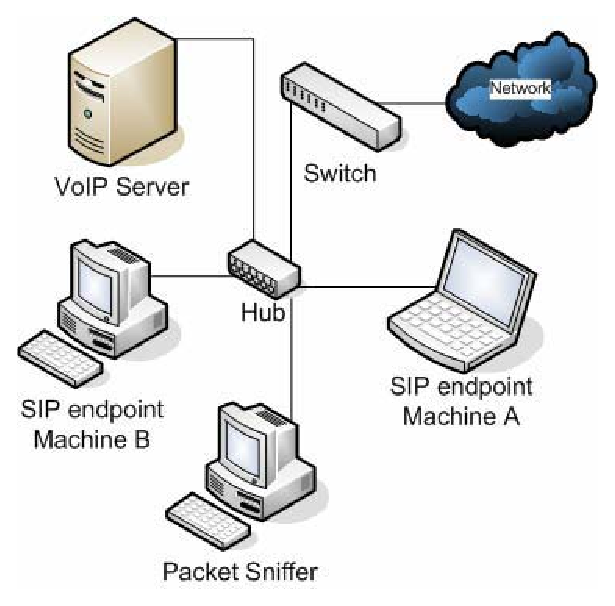
\psfig{file=semi_slike/experiment.eps, width=3in,} % height=1in, width=1in,}
\caption{Postavitev in vloge naprav v eksperimentu.}
\label{fig:setup}
\end{figure}

\begin{figure}
\centering
\begin{verbatim}
tcpdump -nnvvXSs 1514 host \
192.168.1.193 -i eth0 -w voip.cap
\end{verbatim}
\caption{Zajem prometa za/iz naprave klicoče na usmerjevalniku.}
\label{fig:tcpdump}
\end{figure}

Prva ugotovitev je, da lahko s prisluškovanjem znotraj loka\-lnega omrežja brez težav rekonstruiramo celoten klic, vključno z avdio in video komunikacijo (sliki~\ref{fig:call} in ~\ref{fig:audio}). Vendar se tu postavi vprašanje ali je to dovolj dober dokaz na sodišču? Promet na mreži je enostavno ponarediti z npr. napadom replay attack. Večjo stopnjo objektivnosti in verodostojnosti dokaza bi dosegli, če bi ključne informacije klica dejansko našli na fizični napravi, s katere je bil opravljen klic.

\begin{figure*}
\centering
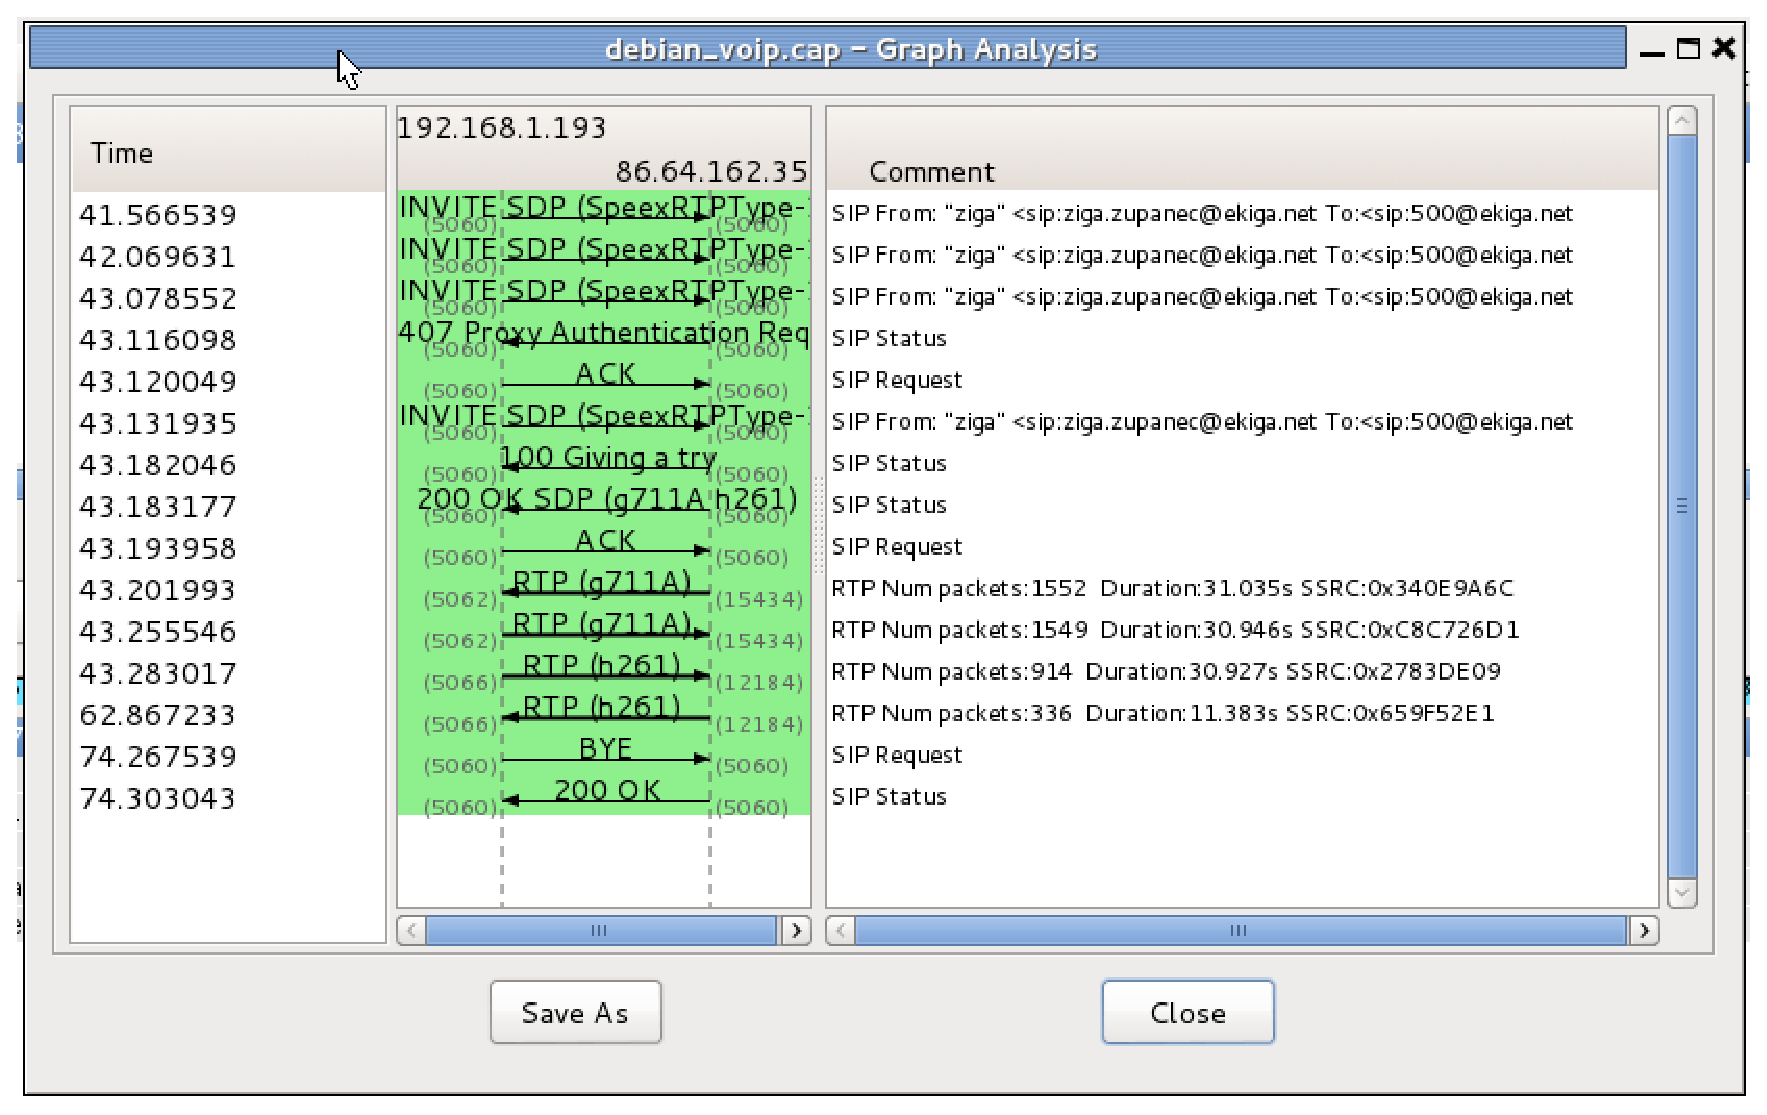
\psfig{file=semi_slike/wireshark_call.eps, width=7in,} % height=1in, width=1in,}
\caption{Vzpostavitev in potek klica.}
\label{fig:call}
\end{figure*}

\begin{figure*}
\centering
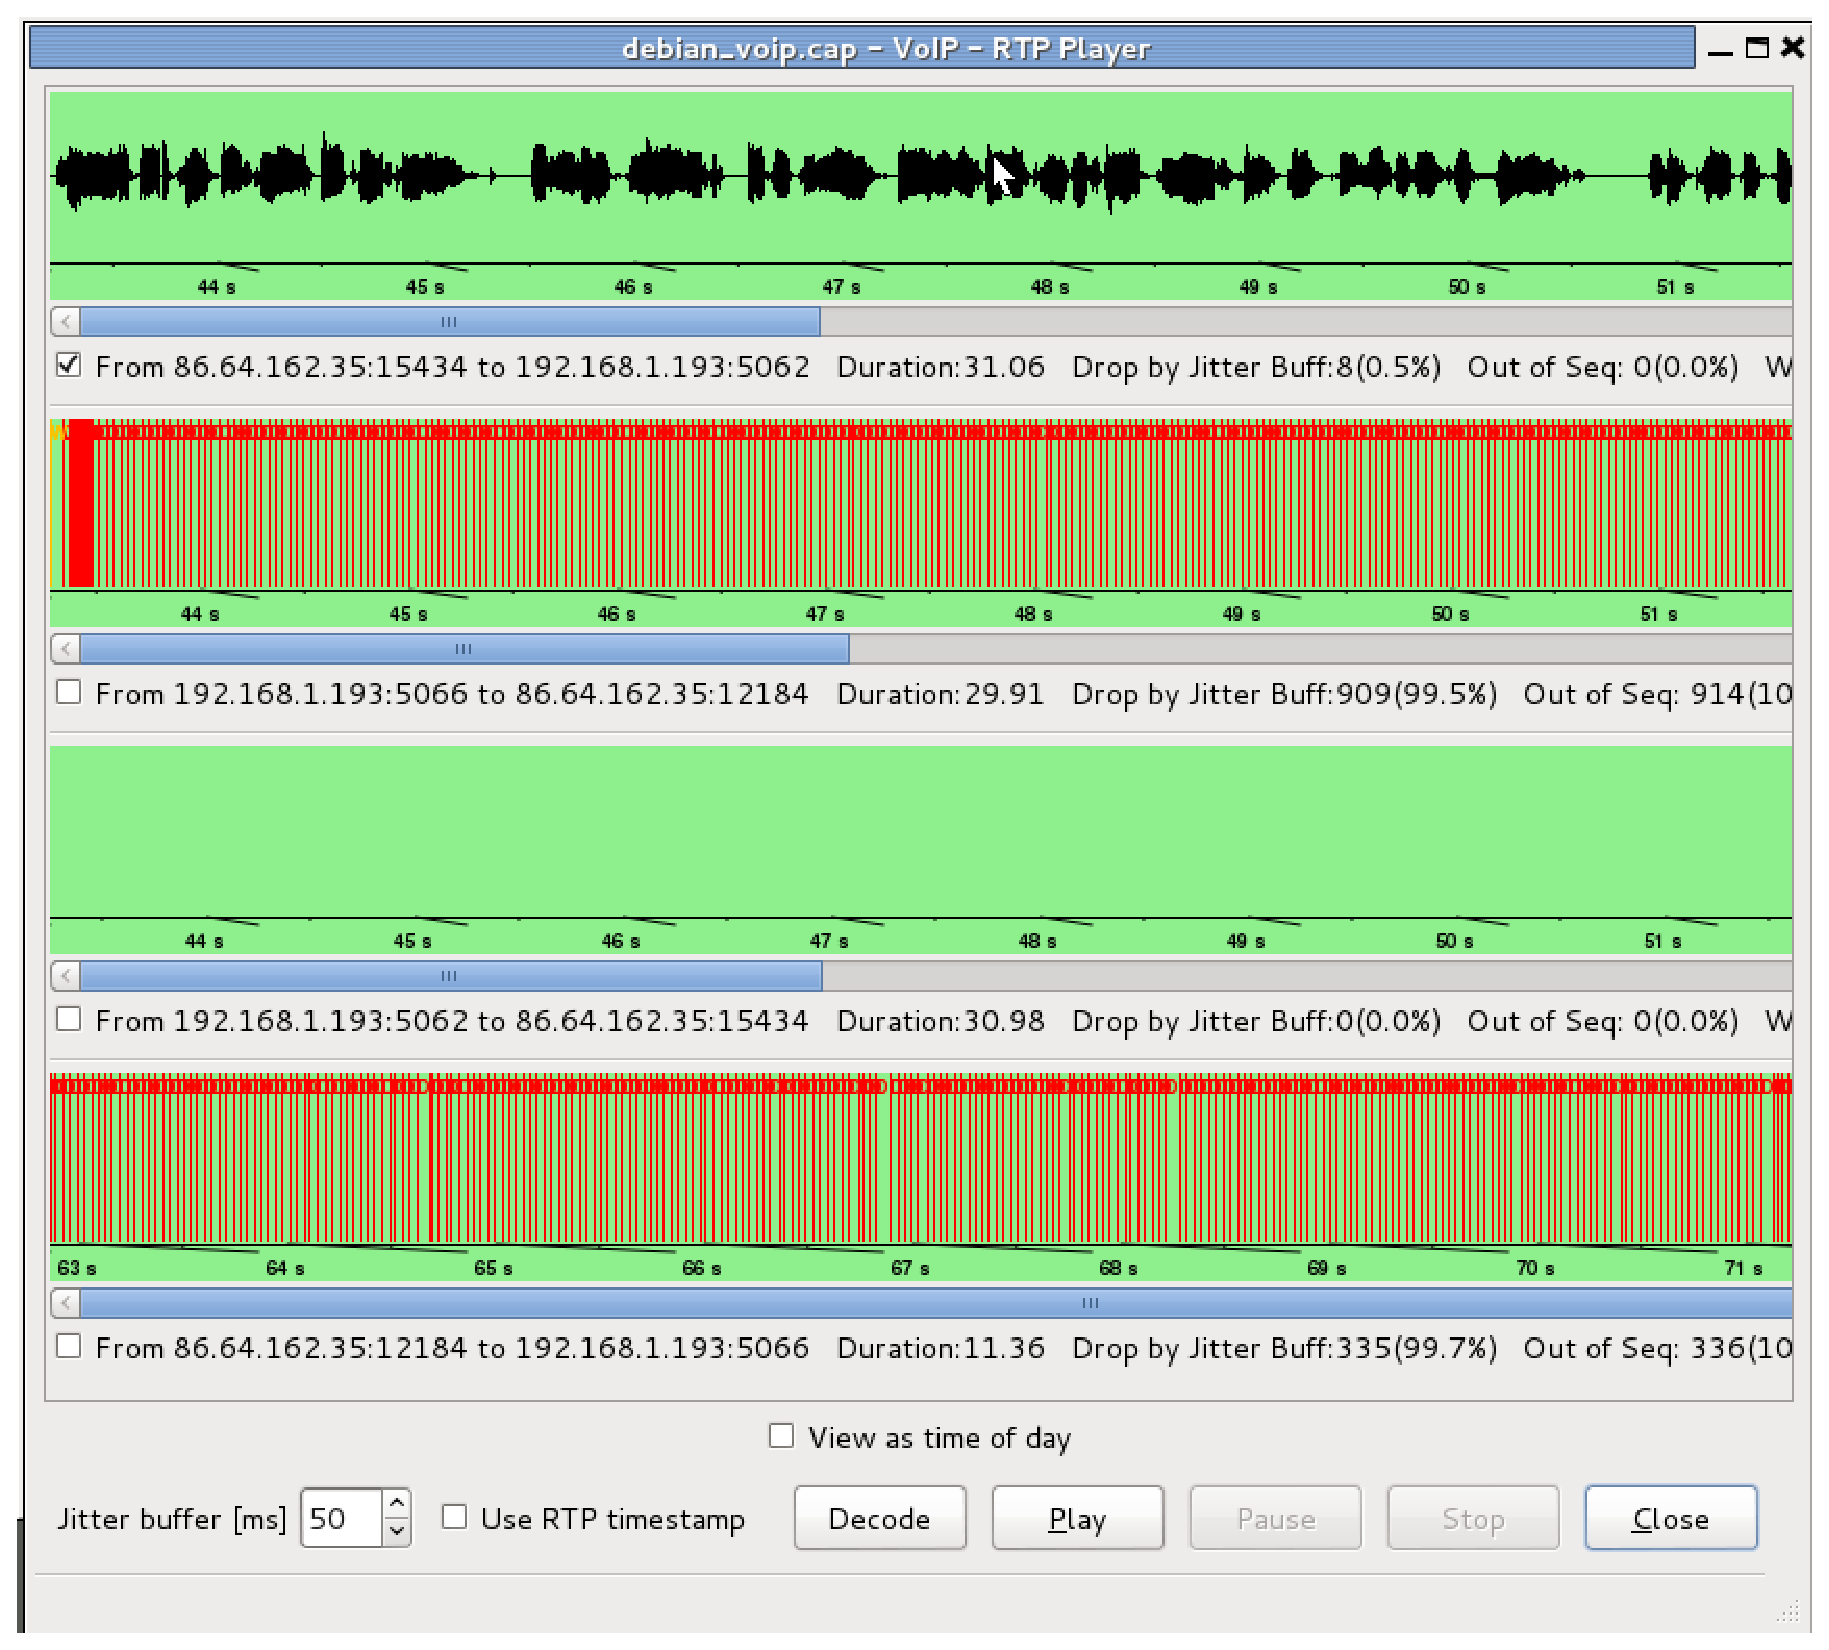
\psfig{file=semi_slike/wireshark_audio.eps, width=7in,} % height=1in, width=1in,}
\caption{Rekonstrukcija zvočnega zapisa s programom wireshark.}
\label{fig:audio}
\end{figure*}

Za potrebe seminarske naloge smo napisali skripto v programskem jeziku python, ki v izpisu diska ali pa v pomnilniškem izpisu poišče ključne elemente seje. Za ključne elemente seje smatramo vse tiste elemente s katerimi je mogoče enolično identificirati določen klic. V konkretnem primeru je ta identifikator:
\\
''Call-ID: 381d54a4-ccd2-e311-90e9-00155d014713@debian32''.

\subsection{Eksperiment 1}

Naša hipoteza je, da bomo na disku odjemalca našli podatke, ki bodo enolično določili klic med vsemi podatki zajetimi na usmerjevalniku. Po opravljenem klicu zajamemo podatke na disku (ukaz~\ref{fig:dd}).

\begin{figure}
\centering
\begin{verbatim}
dd if=/dev/sda of=/mnt/storage/debian.img
\end{verbatim}
\caption{Zajem slike diska.}
\label{fig:dd}
\end{figure}

Na disku nismo našli nobenih sledi, tj. delcev paketov, ki bi lahko predstavljali podatke klica.

\subsection{Eksperiment 2}

V tem eksperimentu pričakujemo, da se bodo podatki, ki enolično določajo klic nahajali v pomnilniškem prostoru odjemalca. Za zajem pomnilnika smo najprej namestili modul fmem, da lahko zajamemo celotno pomnilniško sliko (ukaz~\ref{fig:fmem}).

\begin{figure}
\centering
\begin{verbatim}
dd if=/dev/fmem of=debian_mem.bin bs=1024
\end{verbatim}
\caption{Zajem pomnilniške slike.}
\label{fig:fmem}
\end{figure}

Z našo skripto smo na različnih lokacijah našli niz ''Call-ID'' (slika~\ref{fig:eks2}), kar je dovolj za identifikacijo klica. Našli smo tudi en paket identičen tistemu, ki je bil zajet na usmerjevalniku.

\begin{figure}
\centering
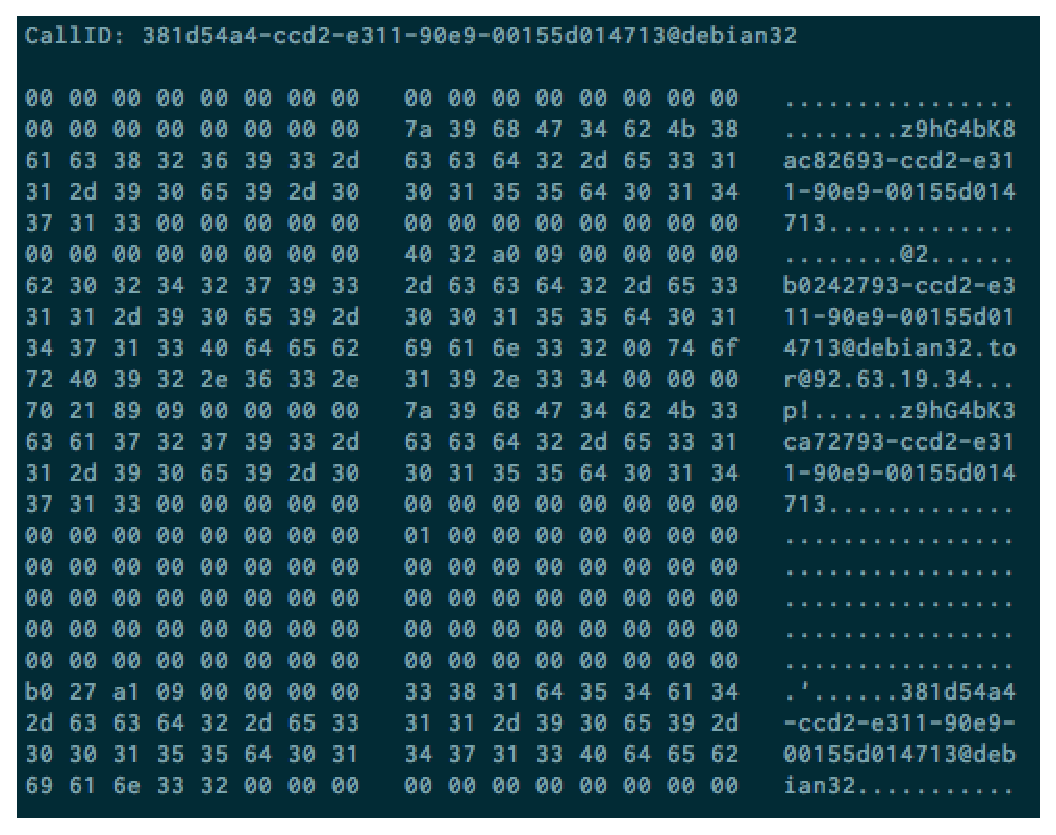
\psfig{file=semi_slike/experiment-2.eps, width=3in,} % height=1in, width=1in,}
\caption{Del pomnilniške slike, kjer smo našli vrednost ''Call-ID''.}
\label{fig:eks2}
\end{figure}

% \subsection{Tables}
% Because tables cannot be split across pages, the best
% placement for them is typically the top of the page
% nearest their initial cite.  To
% ensure this proper ``floating'' placement of tables, use the
% environment \textbf{table} to enclose the table's contents and
% the table caption.  The contents of the table itself must go
% in the \textbf{tabular} environment, to
% be aligned properly in rows and columns, with the desired
% horizontal and vertical rules.  Again, detailed instructions
% on \textbf{tabular} material
% is found in the \textit{\LaTeX\ User's Guide}.
%
% Immediately following this sentence is the point at which
% Table 1 is included in the input file; compare the
% placement of the table here with the table in the printed
% dvi output of this document.
%
% \begin{table}
% \centering
% \caption{Frequency of Special Characters}
% \begin{tabular}{|c|c|l|} \hline
% Non-English or Math&Frequency&Comments\\ \hline
% \O & 1 in 1,000& For Swedish names\\ \hline
% $\pi$ & 1 in 5& Common in math\\ \hline
% \$ & 4 in 5 & Used in business\\ \hline
% $\Psi^2_1$ & 1 in 40,000& Unexplained usage\\
% \hline\end{tabular}
% \end{table}
%
% To set a wider table, which takes up the whole width of
% the page's live area, use the environment
% \textbf{table*} to enclose the table's contents and
% the table caption.  As with a single-column table, this wide
% table will ``float" to a location deemed more desirable.
% Immediately following this sentence is the point at which
% Table 2 is included in the input file; again, it is
% instructive to compare the placement of the
% table here with the table in the printed dvi
% output of this document.
%
%
% \begin{table*}
% \centering
% \caption{Some Typical Commands}
% \begin{tabular}{|c|c|l|} \hline
% Command&A Number&Comments\\ \hline
% \texttt{{\char'134}alignauthor} & 100& Author alignment\\ \hline
% \texttt{{\char'134}numberofauthors}& 200& Author enumeration\\ \hline
% \texttt{{\char'134}table}& 300 & For tables\\ \hline
% \texttt{{\char'134}table*}& 400& For wider tables\\ \hline\end{tabular}
% \end{table*}
% % end the environment with {table*}, NOTE not {table}!
%
% \subsection{Figures}
% Like tables, figures cannot be split across pages; the
% best placement for them
% is typically the top or the bottom of the page nearest
% their initial cite.  To ensure this proper ``floating'' placement
% of figures, use the environment
% \textbf{figure} to enclose the figure and its caption.
%
% This sample document contains examples of \textbf{.eps}
% and \textbf{.ps} files to be displayable with \LaTeX.  More
% details on each of these is found in the \textit{Author's Guide}.
%
% \begin{figure}
% \centering
% \epsfig{file=fly.eps}
% \caption{A sample black and white graphic (.eps format).}
% \end{figure}
%
% \begin{figure}
% \centering
% \epsfig{file=fly.eps, height=1in, width=1in}
% \caption{A sample black and white graphic (.eps format)
% that has been resized with the \texttt{epsfig} command.}
% \end{figure}
%
%
% As was the case with tables, you may want a figure
% that spans two columns.  To do this, and still to
% ensure proper ``floating'' placement of tables, use the environment
% \textbf{figure*} to enclose the figure and its caption.
%
% Note that either {\textbf{.ps}} or {\textbf{.eps}} formats are
% used; use
% the \texttt{{\char'134}epsfig} or \texttt{{\char'134}psfig}
% commands as appropriate for the different file types.
%
% \subsection{Theorem-like Constructs}
% Other common constructs that may occur in your article are
% the forms for logical constructs like theorems, axioms,
% corollaries and proofs.  There are
% two forms, one produced by the
% command \texttt{{\char'134}newtheorem} and the
% other by the command \texttt{{\char'134}newdef}; perhaps
% the clearest and easiest way to distinguish them is
% to compare the two in the output of this sample document:
%
% This uses the \textbf{theorem} environment, created by
% the\linebreak\texttt{{\char'134}newtheorem} command:
% \newtheorem{theorem}{Theorem}
% \begin{theorem}
% Let $f$ be continuous on $[a,b]$.  If $G$ is
% an antiderivative for $f$ on $[a,b]$, then
% \begin{displaymath}\int^b_af(t)dt = G(b) - G(a).\end{displaymath}
% \end{theorem}
%
% The other uses the \textbf{definition} environment, created
% by the \texttt{{\char'134}newdef} command:
% \newdef{definition}{Definition}
% \begin{definition}
% If $z$ is irrational, then by $e^z$ we mean the
% unique number which has
% logarithm $z$: \begin{displaymath}{\log e^z = z}\end{displaymath}
% \end{definition}
%
% \begin{figure}
% \centering
% \psfig{file=rosette.ps, height=1in, width=1in,}
% \caption{A sample black and white graphic (.ps format) that has
% been resized with the \texttt{psfig} command.}
% \end{figure}
%
% Two lists of constructs that use one of these
% forms is given in the
% \textit{Author's  Guidelines}.
%
% \begin{figure*}
% \centering
% \epsfig{file=flies.eps}
% \caption{A sample black and white graphic (.eps format)
% that needs to span two columns of text.}
% \end{figure*}
% and don't forget to end the environment with
% {figure*}, not {figure}!
%
% There is one other similar construct environment, which is
% already set up
% for you; i.e. you must \textit{not} use
% a \texttt{{\char'134}newdef} command to
% create it: the \textbf{proof} environment.  Here
% is a example of its use:
% \begin{proof}
% Suppose on the contrary there exists a real number $L$ such that
% \begin{displaymath}
% \lim_{x\rightarrow\infty} \frac{f(x)}{g(x)} = L.
% \end{displaymath}
% Then
% \begin{displaymath}
% l=\lim_{x\rightarrow c} f(x)
% = \lim_{x\rightarrow c}
% \left[ g{x} \cdot \frac{f(x)}{g(x)} \right ]
% = \lim_{x\rightarrow c} g(x) \cdot \lim_{x\rightarrow c}
% \frac{f(x)}{g(x)} = 0\cdot L = 0,
% \end{displaymath}
% which contradicts our assumption that $l\neq 0$.
% \end{proof}
%
% Complete rules about using these environments and using the
% two different creation commands are in the
% \textit{Author's Guide}; please consult it for more
% detailed instructions.  If you need to use another construct,
% not listed therein, which you want to have the same
% formatting as the Theorem
% or the Definition\cite{salas:calculus} shown above,
% use the \texttt{{\char'134}newtheorem} or the
% \texttt{{\char'134}newdef} command,
% respectively, to create it.
%
% \subsection*{A {\secit Caveat} for the \TeX\ Expert}
% Because you have just been given permission to
% use the \texttt{{\char'134}newdef} command to create a
% new form, you might think you can
% use \TeX's \texttt{{\char'134}def} to create a
% new command: \textit{Please refrain from doing this!}
% Remember that your \LaTeX\ source code is primarily intended
% to create camera-ready copy, but may be converted
% to other forms -- e.g. HTML. If you inadvertently omit
% some or all of the \texttt{{\char'134}def}s recompilation will
% be, to say the least, problematic.
%
\section{Zaključek}
Za forenziko na področju protokola VoIP velja, da je to še precej nerazvito področje. Da ni (prosto dostopnih) orodji za analizo protokola VoIP in, da se tako stanje ohranja naprej bi deloma pripisali dejstvu, da ta orodja verjetno obstajajo, a so v lasti državnih tajnih služb, ki nimajo interesa, da bi ta orodja postala javna. Deloma tako stanje ustreza tudi ponudnikom ter proizvajalcem strojne in programske opreme, saj smo v članku predstavili kako ``ranljiv" je pravzaprav velik del prometa VoIP. Dokler je orodij za analizo prometa VoIP malo, večina proizvajalcev in uporabnikov uživa lažen občutek varnosti, t.i. ``Security through obscurity".

%\end{document}  % This is where a 'short' article might terminate

%ACKNOWLEDGMENTS are optional
% \section{Acknowledgments}
% This section is optional; it is a location for you
% to acknowledge grants, funding, editing assistance and
% what have you.  In the present case, for example, the
% authors would like to thank Gerald Murray of ACM for
% his help in codifying this \textit{Author's Guide}
% and the \textbf{.cls} and \textbf{.tex} files that it describes.

%
% The following two commands are all you need in the
% initial runs of your .tex file to
% produce the bibliography for the citations in your paper.
\bibliography{sigproc-sp}  % sigproc-sp.bib is the name of the Bibliography in this case
\bibliographystyle{abbrv}

%QOS \url{"http://en.wikipedia.org/wiki/Voice_over_IP#Quality_of_service"}
%NAT \url{"http://en.wikipedia.org/wiki/NAT_traversal"}
%TEŽAVE \url{"http://computer.howstuffworks.com/ip-telephony5.htm"}
%OBAMA \url{"http://geeknizer.com/hack-any-cisco-voip-phone/"}

%RAS https://en.wikipedia.org/wiki/Registration,_Admission_and_Status
%H.261 https://en.wikipedia.org/wiki/H.261
%H.323 https://en.wikipedia.org/wiki/H.323
%STUN https://en.wikipedia.org/wiki/STUN
%ekiga http://wiki.ekiga.org/index.php/Manual#H.323_addresses
%nat http://wiki.ekiga.org/index.php/Understanding_NAT/firewall_issues_with_SIP_clients_(eg_ekiga)
% http://webcache.googleusercontent.com/search?q=cache:ZvS3tmAMEvcJ:docwiki.cisco.com/wiki/Cisco_IOS_Voice_Troubleshooting_and_Monitoring_--_H.323-Related_Standards&client=iceweasel-a&hl=en&strip=1

% You must have a proper ".bib" file
%  and remember to run:
% latex bibtex latex latex
% to resolve all references
%
% ACM needs 'a single self-contained file'!
%
%APPENDICES are optional
%\balancecolumns
% \appendix
% %Appendix A
% \section{Headings in Appendices}
% The rules about hierarchical headings discussed above for
% the body of the article are different in the appendices.
% In the \textbf{appendix} environment, the command
% \textbf{section} is used to
% indicate the start of each Appendix, with alphabetic order
% designation (i.e. the first is A, the second B, etc.) and
% a title (if you include one).  So, if you need
% hierarchical structure
% \textit{within} an Appendix, start with \textbf{subsection} as the
% highest level. Here is an outline of the body of this
% document in Appendix-appropriate form:
% \subsection{Introduction}
% \subsection{The Body of the Paper}
% \subsubsection{Type Changes and  Special Characters}
% \subsubsection{Math Equations}
% \paragraph{Inline (In-text) Equations}
% \paragraph{Display Equations}
% \subsubsection{Citations}
% \subsubsection{Tables}
% \subsubsection{Figures}
% \subsubsection{Theorem-like Constructs}
% \subsubsection*{A Caveat for the \TeX\ Expert}
% \subsection{Conclusions}
% \subsection{Acknowledgments}
% \subsection{Additional Authors}
% This section is inserted by \LaTeX; you do not insert it.
% You just add the names and information in the
% \texttt{{\char'134}additionalauthors} command at the start
% of the document.
% \subsection{References}
% Generated by bibtex from your ~.bib file.  Run latex,
% then bibtex, then latex twice (to resolve references)
% to create the ~.bbl file.  Insert that ~.bbl file into
% the .tex source file and comment out
% the command \texttt{{\char'134}thebibliography}.
% % This next section command marks the start of
% % Appendix B, and does not continue the present hierarchy
% \section{More Help for the Hardy}
% The acm\_proc\_article-sp document class file itself is chock-full of succinct
% and helpful comments.  If you consider yourself a moderately
% experienced to expert user of \LaTeX, you may find reading
% it useful but please remember not to change it.
% \balancecolumns
% % That's all folks!
\end{document}
